% arara: lualatex
% !TEX TS-program = LuaLaTeX


\documentclass{coderdojo}

\worksheet{8}{Working with Lists I}

\newcommand\contentsitem[2]{
	\item \hyperref[#1]{\color{section}\bfseries #2}
}

\usepackage{wrapfig}
\usepackage{float}

\newcommand\TODO[1]{
\begin{itemize}
\item[\todoSymbol] \color{todo} #1
\end{itemize}}


\newcommand\TEST[1][\bf Test your code!]{
	\centerline{\tikz\node[starburst, fill=yellow, draw=red, line width=2pt,align=center] {#1};}
}

\newcommand\TESTSMALL[2][\bf Test your code!]{
{\tikz[scale=#2]\node[starburst, fill=yellow, draw=red, line width=2pt,align=center] {#1};}
}

\usetikzlibrary{decorations,
decorations.pathreplacing,decorations.pathmorphing}

\newenvironment{clist}
{\begin{list}{$\bullet$}{\setlength{\leftmargin}{6pt}}}
{\end{list}}

% postit
\tikzstyle{postit}=[fill=yellow!50,draw,thick,
decorate, drop shadow,
decoration={random steps,segment length=3pt,amplitude=1pt},
text width=4cm, font=\smaller]

\tikzstyle{postitnumber}=[inner sep=2pt,fill=yellow!50,draw,circle,font={\bf\smaller[3]}]

\newcommand\postit[2][]{\tikz\node[postit,#1] {#2};}


\begin{document}
\maketitle

\section*{Introduction}

This week we are going to something different.  We are going take a closer look at python lists. We have used lists before, in our graphical {\em Take Away} game to store the messages that we wanted to display, but we need to look at lists more carefully if we are going to develop more complicated programmes/games.

\subsection*{So what is a list? }

\begin{center}
	\begin{tikzpicture}
\node[fill=yellow!10,drop shadow, rounded corners=6pt] (M)
	{\Large\bfseries A list is an ordered collection of data values};
\node[postit] at (-4,-3) (O) {{\bf ordered} does not mean sorted. Instead it means that we know the order in which the data values are arranged. \\
So, given order, we can ask for 
the 0\textsuperscript{th}, 
the 1\textsuperscript{st}, 
the 2\textsuperscript{nd}, etc. data value. 
};
\node[postit] at (1,-2) (C) {{\bf collection} means that we can store zero, one, or many data values.};
\node[postit] at (6,-3) (D) {{\bf data values} can be any valid data -- numbers, strings, or more fancy data such as our turtles. And there is no restriction that the data values are the same type.};

\tikzstyle{e}=[very thick, -latex]
\draw[e] (O) -- ($(M.south)+(-1.9,0.0)$);
\draw[e] (C) -- ($(M.south)+(0.5,0.0)$);
\draw[e] (D) -- ($(M.south)+(4,0.0)$);

\end{tikzpicture}
\end{center}



\subsection*{How To Create a List?}

Creating a list is very simple. You simple put your data values inside square brackets, and separate each value with a comma. So, for example,

\begin{itemize}
\item \code{list1 = [0, 1, 2, 3, 4, 5]}

Creates a list storing the integers from 0 to 5 inclusive.

\item \code{list2 = ["My", "name","is", "bob"]}

Lists can store any data type --- the above list stores 4 strings.

\item \code{list3 = [107, 0.4, "hello", [2,3]]}

Lists can store a mixture of data types --- including other lists!
The above list stores four data values each of a different type:
	\begin{itemize}
	\item \code{107} is an integer \hfill in python terminology this is an \code{int}.
	\item \code{0.4} is a floating point number since it has a decimal point
	\\\mbox{}\hfill
	 \hfill in python terminology this is a \code{float}.
	 \item \code{"hello"} is a string
	 \hfill in python terminology this is a \code{str}.
	 \item \code{[2,3]} is a list containing two integers.
	\end{itemize}

\end{itemize}

\section*{How big is a  List ?}

To determine how many data values are in a list we use the command \code{len}. For example the code

\hspace*{3cm}\begin{minipage}{\textwidth}
\code{list3 = [107, 0.4, "hello", [2,3]]}\\
\code{print(len(list3))}
\end{minipage}

\vspace{3pt}
outputs \code{4} because the list contains four data values --- an integer, a float, a string, and a list.

\section*{How To Access Data Stored in a List ?}

We have three ways to get at the data that is stored in a list 
\begin{itemize}
\item {\bf indexing} --- count up positions from the left, starting at zero.
\item {\bf negative indexing} --- count down positions from the right, starting at negative one.
\item {\bf slicing} --- given a pair of indexes, extract a sub list from a list.
%\item {\bf slicing with stride} --- a more powerful version of slicing.
\end{itemize}

Each method is covered in the following sections.

\subsection*{Indexing}

When we create a list we give it a name --- I used \code{list1}, \code{list2}, etc in the previous page, but you can come up with much better names that that\footnote{In programming we put a lot of effort in to generating sensible, informative names for our variables. It makes our code much easier to read.}. Using the list name and square brackets\footnote{square brackets \code{[]} are called {\bf index operator}.}  we can access any value in the list, counting from the left and starting with zero.
For example, the code

\vspace{6pt}
\centerline{\code{a = ['foo', 'bar', 'baz', 'qux', 'quux', 'corge']}}

creates the list 

\vspace{6pt}
\centerline{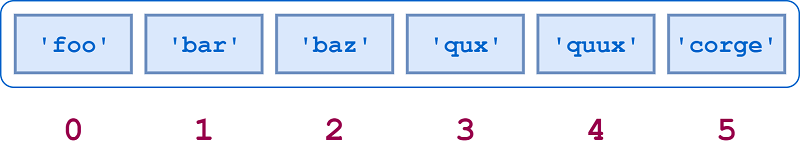
\includegraphics[scale=.6]{python-list-01.png}}

Then 
\begin{itemize}
\item \code{a[0]} refers to the string \code{'foo'}.
\item \code{a[1]} refers to the string \code{'bar'}.
\item[] \hspace{3cm}$\vdots$
\item \code{a[5]} refers to the string \code{'corge'}.
\end{itemize}
\mbox{}\hfill\raisebox{1cm}[0pt][0pt]{\postit[text width=7cm]{The number in the square brackets is called the {\bf index} and it needs to be an integer.\\[12pt]
 So something like \code{a["2"]} will not work.\\[12pt]
 
If the index does not refer to a valid position in the list a \code{IndexError} will occur.
 }}

\newpage
\subsection*{Negative Indexing} 

Python has this cool feature --- if we pass a negative integer as an index then it will start counting from the right, starting with negative 1.

\vspace{6pt}
\centerline{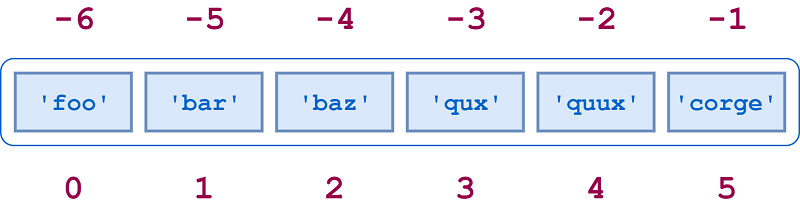
\includegraphics[scale=.6]{python-list-02.png}}

So 
\begin{itemize}
\item \code{a[-1]} refers to the string \code{'corge'}.
\item \code{a[-2]} refers to the string \code{'quux'}.
\item[] \hspace{3cm}$\vdots$
\item \code{a[-6]} refers to the string \code{'foo'}.
\end{itemize}

\subsection*{Slicing}

If we put two integers inside the square brackets, as in \code{[m:n]} we don't just get a single data value back --- we get a sub-list back, of all data values from position \code{m} up to but not including position \code{n}. 

If either, or both \code{m} and \code{n} can be missing then the sub-list extends to start or end of the original list.

For example, given the code

\vspace{6pt}
\centerline{\code{a = ['well', 'good', 'google', 'book', 'red', 'blue']}}

then 
\begin{itemize}
\item \code{a[2:5]} returns sub-list \code{['google', 'book', 'red']}

Returned list was a sub-list of the original list, starting with data value at index \code{2} and up to but not including data value at index \code{5}.

\item \code{a[2:]} returns sub-list \code{['google', 'book', 'red', 'blue']}

(Note \code{n} was missing.)

Returned list was a sub-list of the original list, starting with data value at index \code{2} and up to the end of original list.

\item \code{a[:5]} returns sub-list \code{['well', 'good', 'google', 'book', 'red']}

(Note \code{m} was missing.)

Returned list was a sub-list of the original list, starting at start of original list and up to but not including data value art index \code{5}.

\item \code{a[:]} returns sub-list \code{['well', 'good', 'google', 'book', 'red', 'blue']}

(Note \code{m} was missing.)

Returned list was a sub-list of the original list,  starting at start of original list and ending at end, i.e., the entire list.
\end{itemize}
%
%\subsection*{Slicing with Stride}
%
%\mbox{}\hfill\parbox{.7\textwidth}{\em\smaller For completeness I will mention slicing with stride here. We won't be using this for a while so feel free to ignore this for now.}
%
%\vspace{12pt}
%If we have three integers inside the square brackets, \code{[m:n:k]} then this builds up a sub-list from data values starting at index \code{m} and up to but not including the data value at index \code{n} but only picking every \code{k} value.
%

%TODO insert nested list see 
%\centerline{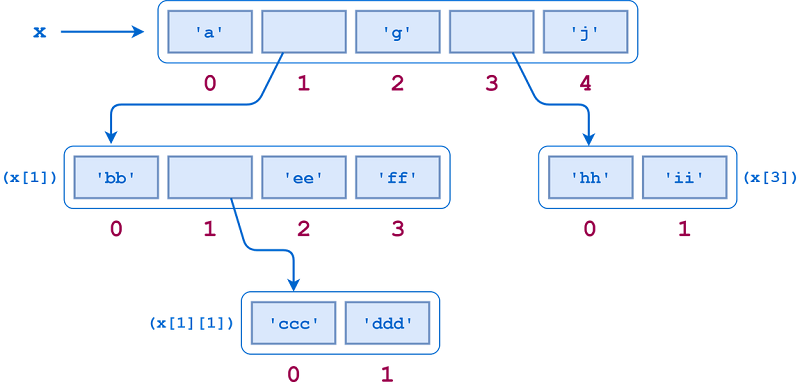
\includegraphics[scale=.8]{python-list-03.png}}

\newpage
\section*{Programming Tasks} 

%: list_tasks_start
\TODO {Open a new file and type in the following code. We will use this as a starting point for the following exercises.}

\codeandoutput{title={\code{list_tasks_start.py}}}{1}{20}{code}{list_tasks.py}{
\ttfamily\smaller 
Generated data is\\

[63, 2, 27, 22, 73, 67, 89, 8, 42, 2]
}

%: list_tasks_1
\TODO {Save your \code{list_tasks_start.py} as \code{list_tasks_1.py}
and add code to print out the data value at index 5.}

\mbox{}\hfill\tikz\node[minimum width=5cm,fill=yellow!10,drop shadow,rounded corners] {67};

%: list_tasks_2
\TODO {Save your \code{list_tasks_start.py} as \code{list_tasks_2.py}
and add code to print out the data values, with one value per line --- you need a for loop.}

\mbox{}\hfill\tikz\node[align=left,minimum width=5cm,fill=yellow!10,drop shadow,rounded corners]
{63\\2\\27\\22\\73\\67\\89\\8\\42\\2};

%: list_tasks_3
\TODO {Save your \code{list_tasks_start.py} as \code{list_tasks_3.py}
and add code to print out the data values, with one value per line but in reverse order.}

\mbox{}\hfill\tikz\node[align=left,minimum width=5cm,fill=yellow!10,drop shadow,rounded corners] 
{2\\42\\8\\89\\67\\73\\22\\27\\2\\63};

\newpage

%: list_tasks_4
\TODO {Save your \code{list_tasks_start.py} as \code{list_tasks_4.py}
and add code to print out the maximum data value in the list.}

\mbox{}\hfill\tikz\node[align=left,minimum width=5cm,fill=yellow!10,drop shadow,rounded corners] 
{89};


%: list_tasks_5
\TODO {Save your \code{list_tasks_start.py} as \code{list_tasks_5.py}
and add code to print out the minimum data value in the list.}

\mbox{}\hfill\tikz\node[align=left,minimum width=5cm,fill=yellow!10,drop shadow,rounded corners] 
{2};

%: list_tasks_6
\TODO {Save your \code{list_tasks_start.py} as \code{list_tasks_6.py}
and add code to print out the difference between the maximum value and the minimum data value in 
the list.}

\mbox{}\hfill\tikz\node[align=left,minimum width=5cm,fill=yellow!10,drop shadow,rounded corners] 
{87};

%: list_tasks_7
\TODO {Save your \code{list_tasks_start.py} as \code{list_tasks_7.py}
and add code to print out the index of the maximum value in the list. 
\\If the maximum value appears more than once, then print out index of first occurrence. 
}

\mbox{}\hfill\tikz\node[align=left,minimum width=5cm,fill=yellow!10,drop shadow,rounded corners] 
{6};

%: list_tasks_8
\TODO {Save your \code{list_tasks_start.py} as \code{list_tasks_8.py}
and add code to print out the index of the minimum value in the list. 
\\If the minimum value appears more than once, then print out index of first occurrence. 
}

\mbox{}\hfill\tikz\node[align=left,minimum width=5cm,fill=yellow!10,drop shadow,rounded corners] 
{0};


%: list_tasks_9
\TODO {Save your \code{list_tasks_start.py} as \code{list_tasks_9.py}
and add code to print out the total of the data values in the list.
}

\mbox{}\hfill\tikz\node[align=left,minimum width=5cm,fill=yellow!10,drop shadow,rounded corners] 
{395};

%: list_tasks_10
\TODO {Save your \code{list_tasks_start.py} as \code{list_tasks_10.py}
and add code to print out the total of all of the even data values minus the total of the odd data values in the list.
}

\mbox{}\hfill\tikz\node[align=left,minimum width=5cm,fill=yellow!10,drop shadow,rounded corners] 
{-243};

%: list_tasks_11
\TODO {Save your \code{list_tasks_start.py} as \code{list_tasks_11.py}
and add code to print out the second largeest data value in the list.}

\mbox{}\hfill\tikz\node[align=left,minimum width=5cm,fill=yellow!10,drop shadow,rounded corners] 
{73};

Hints:
\begin{itemize}
\item Use \code{for k in range(len(data)):}\\
To have a loop variable, \code{k}, that runs over the indexes needed to access all the data values in list \code{data}.
\item Use \code{for d in data:}\\
To have a loop variable, \code{d}, that runs over the data values in the list \code{data}.
\item Use \code{for k,d in enumerate(data):}\\
To have two loop variables, \code{k} and \code{d}, that runs over the indexes and the data values in the list \code{data}.

\end{itemize}
\newpage
\section*{Harder Programming Tasks}

Some extra problems, again using the same generated dataset:

\vspace{6pt}
\centerline{\tikz
\node[fill=yellow!10,drop shadow, rounded corners=6pt] (M)
	{\Large\bfseries [63, 2, 27, 22, 73, 67, 89, 8, 42, 2]
};}

%: list_tasks_extra_1
\TODO {Save your \code{list_tasks_start.py} as \code{list_tasks_extra_1.py}
and add code to print out the data value of the number that appears to the left of the maximum value in the list.\\
If the maximum value appears more than once, then print out index of first occurrence.
If maximum value appears in index 0 then return \code{None}
}

\mbox{}\hfill\tikz\node[align=left,minimum width=5cm,fill=yellow!10,drop shadow,rounded corners] 
{67};


%: list_tasks_extra_2
\TODO {Save your \code{list_tasks_start.py} as \code{list_tasks_extra_2.py}
and add code to print out length of the longest sublist of increasing data values in the list.\\

For example, sub-lists \code{[2,27]}, \code{[22,73]} are both sub-list with increasing data values. 
}

\mbox{}\hfill\tikz\node[align=left,minimum width=5cm,fill=yellow!10,drop shadow,rounded corners] 
{2};

%: list_tasks_extra_3
\TODO {Save your \code{list_tasks_start.py} as \code{list_tasks_extra_3.py}
and add code to print out the longest sublist of increasing data values in the list {\bf where you can skip over  data values that result in decreasing value}.\\

For example, sub-list \code{[2,22,73]}, has increasing data values, and is of length 3. It was obtained by starting at \code{2} but skipping over data value \code{27}.
}

\mbox{}\hfill\tikz\node[align=left,minimum width=5cm,fill=yellow!10,drop shadow,rounded corners] 
{[2,22,67,89]};

\end{document}

